\subsection{VHDL Code}
%insert code here
 Die Statemachine der Motorkühlung ist in drei teile aufgeteilt, dem Zustandsspeicher ``STATE\_REGISTER'', der Übergangsfunktion ``INPUT\_LUT'' und der Ausgangsfunktion ``OUTPUT\_LUT''. Das Signal ``S'' besteht aus einem Vector mit einer drei Bit Länge, dieser steht für die Sensoren der Pumpen. Jede Pumpe gibt ein High oder Low Signal aus, je nachdem ob sie  Funktionstüchtig ist oder nicht. Da dieses Signal  asynchron ist, wird es durch zwei D-Flipflops geführt um Synchronisiert und gepuffert zu werden. Erst nach zwei Taktcyclen empfängt die Übergangsfunktion die Eingabe und setzt nächsten State im Zustandsspeicher. Daraufhin reagiert die Ausgabe Funktion und schaltet je nach zustand die LEDs ein oder aus. Durch diese drei Flipflops wird das Signal um insgesamt drei Taktcyclen verlangsamt.
 
\lstinputlisting[language=VHDL]{img/COOLANT_MONITOR.VHDL}


\subsection{Simulation}
%insert sim here


% grafik einbinden
\begin{figure}[H]
    \begin{center}
        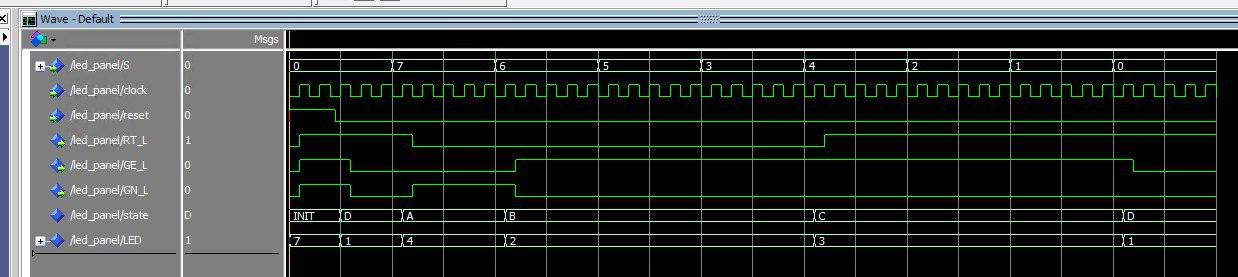
\includegraphics[width=1\textwidth]{img/motorsim.jpg}
        \caption{Simulation}
        \label{fig:A1_sim}
    \end{center}
\end{figure}

Die Startbedingung wird durch den Reset Eingang erfüllt, beim Start des Automat ist der Resetpin auf eins und setzt den Start state $Q_0$ auf ``INIT'' um einen definierten zustand zu erhalten.

\subsection{Auswertung}
